\chapter{Perancangan}
\label{chap:Perancangan}

Pada bab 4 akan dibahas mengenai perancangan seperti diagram \textit{sequence} kelas secara rinci dan perancangan antarmuka.

%Perancangan Diagram Sequence
\section{Diagram \textit{Sequence}}
\label{lab:Diagram Sequence}
\hspace{0.5cm} Diagram \textit{sequence} merupakan diagram yang menggambarkan interkasi antar objek dalam suatu skenario. Gambar diagram \textit{sequence} dapat dilihat pada gambar ~ref{fig:sequence lokasi perangkat} sampai ~ref{fig:sequence rute}. 

% Sequence mendapat lokasi perangkat
\begin{figure}[h]
	\centering
		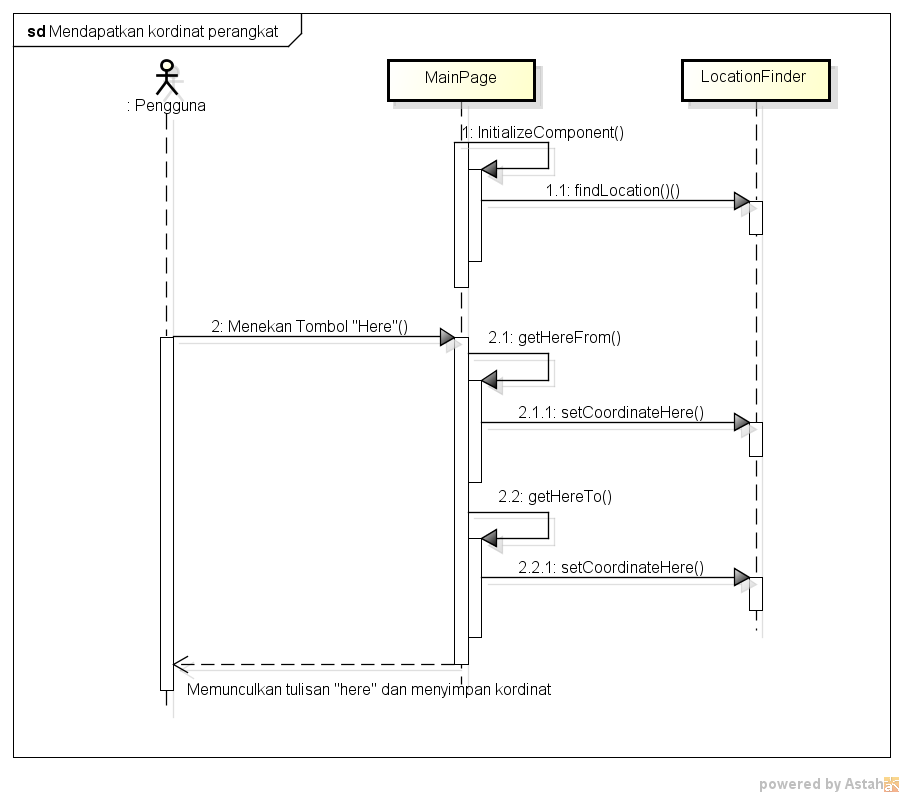
\includegraphics[scale=0.4]{Gambar/sequence/MendapatkanKordinatPerangkat}
	\caption{Diagram \textit{sequence} Mendapatkan Kordinat perangkat}
	\label{fig:sequence lokasi perangkat}
\end{figure}

\hspace{0.5cm} Diagram ~\ref{fig:sequence lokasi perangkat} merupakan diagram \textit{sequence} untuk memilih lokasi dengan lokasi perangkat berada. Diagram menunjukan bahwa setelah aplikasi dibuka maka aplikasi akan mencari dahulu lokasi perangkat. Lalu setelah aplikasi terbuka jika pengguna ingin memilih lokasi tersebut sebagai lokasi asal maka pengguna harus menekan tombol "here". Setelah tombol "here" ditekan maka kelas MainPage akan mengambil nilai \textit{Latitude} dan nilai \textit{Longitude} dari kelas LocatonFinder. Setelah lokasi didapatkan maka akan muncul tulisan "here" pada masukan di kelas MainPage.

% Sequence mendapat lokasi dari peta
\begin{figure}[h]
	\centering
		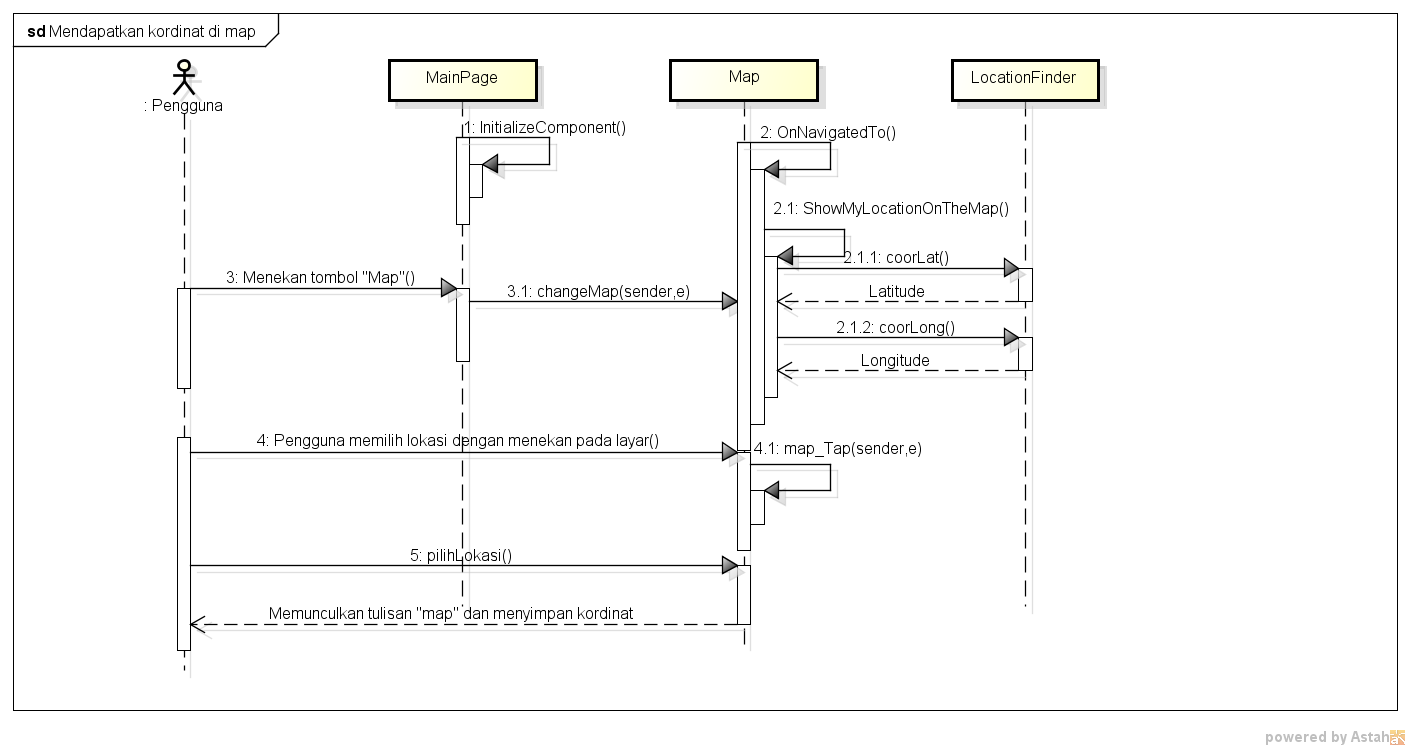
\includegraphics[scale=0.4]{Gambar/sequence/MendapatkanKordinatDiMap}
	\caption{Diagram \textit{sequence} Mendapatkan Kordinat pada Peta}
	\label{fig:sequence lokasi pada peta}
\end{figure}

\hspace{0.5cm} Diagram ~\ref{fig:sequence lokasi pada peta} merupakan diagram \textit{sequence} untuk memilih lokasi. Diagram menunjukan bahwa setelah aplikasi dibuka maka pengguna dapat menekan tombol "map". Setelah tombol "map" ditekan maka halaman akan dialihkan ke kelas Map. Di kelas "Map" pengguna dapat memilih lokasi dengan memilih lokasi pada peta dan memanggil \textit{method map\_tap}, lalu setelah pengguna memilih tempat pengguna akan menekan tombol Pilih Lokasi yang akan memanggil \textit{method pilihLokasi}. Lokasi yang dipilih pengguna akan disimpan di kelas MainPage dan pada masukan akan tertulis "map". 

\hspace{0.5cm} Diagram ~\ref{fig:sequence rute} merupakan diagram \textit{sequence} untuk mencari rute. Diagram menunjukan bahwa setelah aplikasi dibuka maka aplikasi akan melakukan inisialisasi. Selanjutnya pengguna juga dapat memasukan kata kunci untuk masukan asal dan tujuan (masukan dapat juga dari peta atau lokasi perangkat sesuai diagram ~\ref{fig:sequence lokasi perangkat} dan ~\ref{fig:sequence lokasi pada peta}) lalu memanggil \textit{method startRoute}. Jika masukan yang didapat berupa kata kunci maka akan dilakukan pemeriksaan apakah kordinat untuk kata kunci tersebut tersedia. Pemeriksaan dilakukan dengan melakukan pemanggilan Kiri API. Tahap pemanggilan meliputi pemangilan \textit{method GetStringAsync} lalu mengjadikan objek kembaliannya dengan \textit{method Deselialize}. Jika sudah didapat dan hasilnya lebih dari satu maka akan dipanggil \textit{method getListItem} yang akan menampilkan daftar pilihan ke pengguna untuk dipilih. Pengguna dapat memilih tempat sesuai tempat asal maupun tujuan yang diinginkan. Setelah lokasi asal dan lokasi tujuan didapat maka kelas MainPage akan mengarahkan ke kelas Route untuk menampilkan hasilnya. Kelas Route akan memanggil \textit{method OnNavigatedTo} yang bertujuan untuk mendapatkan lokasi asal dan lokasi tujuan. Setelah itu akan memanggil \textit{method Find} lalu mengembalikan rute yang ditemukan kepada pengguna.

\newpage

% Sequence mendapat rute
\begin{figure}[h]
	\centering
		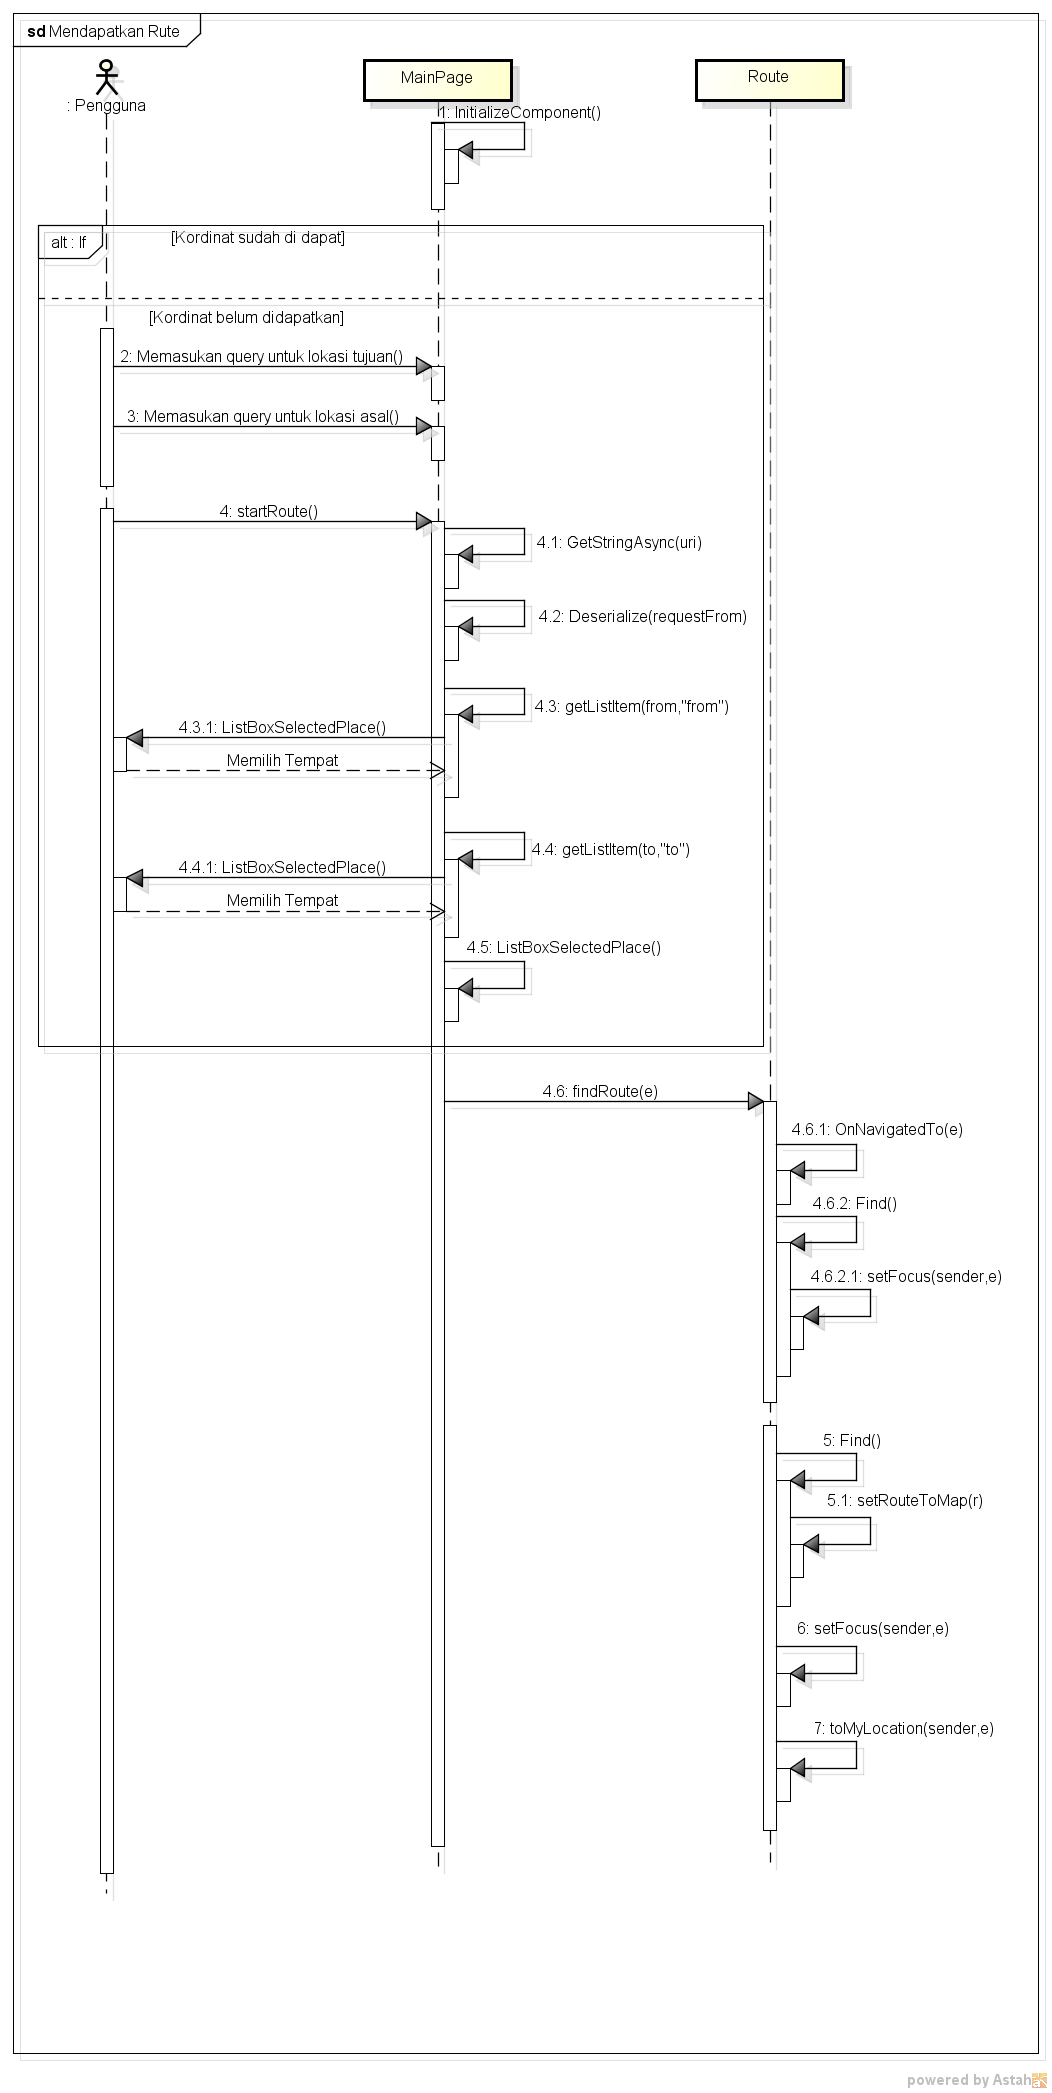
\includegraphics[scale=0.5]{Gambar/sequence/MendapatkanRute}
	\caption{Diagram \textit{sequence} Mendapatkan Rute}
	\label{fig:sequence rute}
\end{figure}


\newpage

%Perancangan Kelas
\section{Perancangan Kelas}
\label{lab:Perancangan Kelas}
\hspace{0.5cm} Pada sub bab ini akan dibahas mengenai deskripsi kelas secara rinci pada aplikasi Pencari Rute Kendaraan Umum untuk Windows Phone. Untuk lebih jelas mengenai kelas yang ada pada aplikasi ini, penulis menyajikan gambar diagram kelas yang dapat dilihat pada  gambar ~\ref{fig:kelas}. 

% Kelas
\begin{figure}[h]
	\centering
		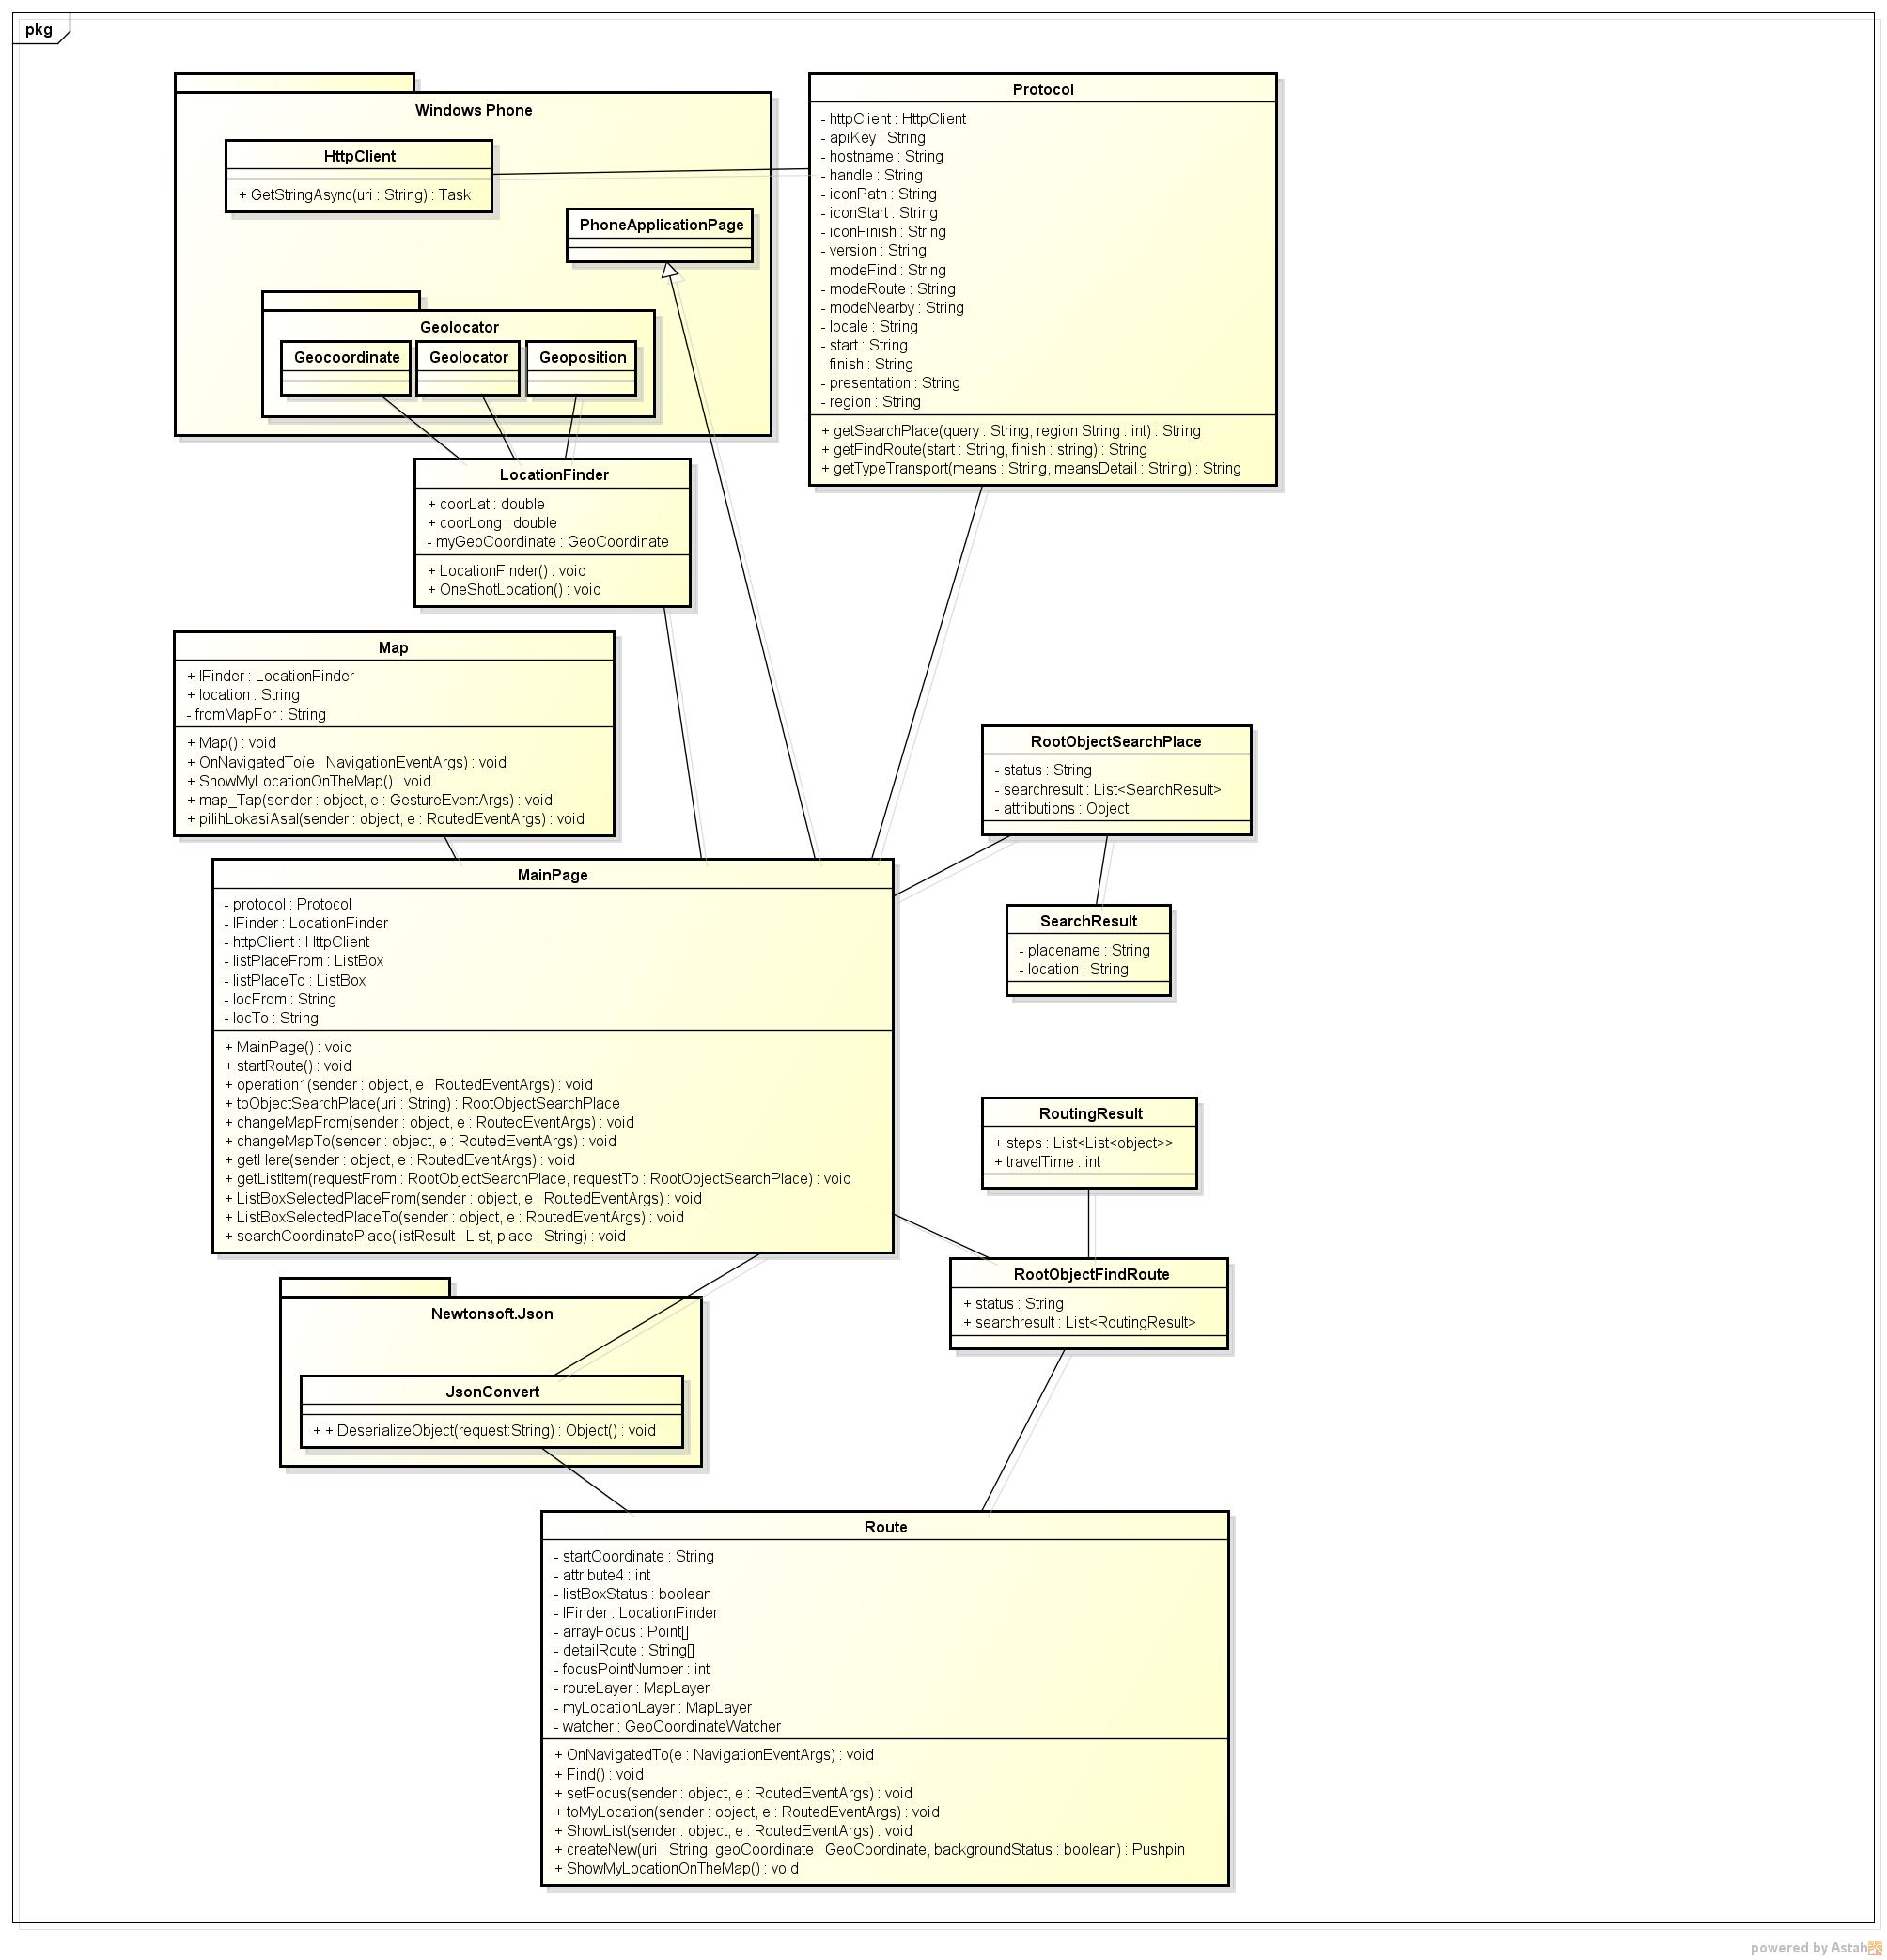
\includegraphics[scale=0.2]{Gambar/useCase_dan_Class/class4}
	\caption{Diagram Kelas}
	\label{fig:kelas}
\end{figure}


%Kelas PhoneApplicationPage
\subsection{Kelas \textit{PhoneApplicationPage}}
\label{lab:Kelas PhoneApplicationPage}
\hspace{0.5cm} \textit{PhoneApplicationPage} merupakan kelas bawaan Windows Phone yang menangani interksi pengguna dengan aplikasi dan siklus hidup aplikasi.

%Kelas MainPage
\subsection{Kelas \textit{MainPage}}
\label{lab:Kelas MainPage}
\hspace{0.5cm} \textit{MainPage} merupakan kelas kelas turunan dari kelas \textit{PhoneApplicationPage} yang menangani interaksi langsung antara halaman aplikasi dengan pengguna. Pada kelas ini akan ditaruh kontrol yang diperlukan. Berikut adalah penjelasan atribut-atribut yang dimiliki kelas ini:
\begin{enumerate}
	\item protocol bertipe Protocol untuk mendapatkan URL yang digunakan dalam permintaan ke Kiri API.
	\item lFinder bertipe LocationFinder yang akan menampung objek untuk pencarian lokasi.
	\item httpClient bertipe HttpClient merupakan objek yang akan mengurus permintaan dan kembalian dari Kiri API.
	\item locationFrom bertipe string untuk menampung kordinat awal.
	\item locationTo bertipe string untuk menampung kordinat tujuan.
	\item city bertipe kumpulan String untuk menampung kota yang didukung oleh layanan Kiri.
	\item myCity bertipe String untuk menampung kode kota sesuai Kode Penerbangan IATA.
	\item backgroundWorker bertipe BackgroundWorker untuk mengurus pencarian lokasi di belakang layar.
\end{enumerate}

Berikut adalah penjelasan metode-metode yang dimiliki kelas ini:
\begin{enumerate}
	\item Konstruktor MainPage digunakan sebagai konstruktor pada kelas MainPage.
	\item Metode OnNavigatedTo digunakan untuk mendapatkan lokasi dari peta dengan masukan NavigationEventArgs.
	\item Metode startRoute digunakan untuk mendapatkan masukan pengguna lalu mengkalkulasi masukan tersebut menjadi kordinat asal dan tujuan lalu mengirimkannya ke kelas Route.
	\item Metode changeMapFrom digunakan untuk berpindah ke halaman mapFrom.
	\item Metode changeMapTo digunakan untuk berpindah ke halaman mapTo.
	\item Metode getHereFrom digunakan untuk mendapatkan kordinat dimana perangkat berada dan menyimpan nilainya di atribut locationFrom.
	\item Metode getHereTo digunakan untuk mendapatkan kordinat dimana perangkat berada dan menyimpan nilainya di atribut locationTo.
	\item Metode getListItem digunakan untuk membuat listBox lalu menampilkan ke pengguna. 
	\item Metode ListBoxSelectedPlace digunakan untuk mendapatkan tempat asal yang dipilih pengguna. Metode ini memiliki parameter objek dan \textit{event SelectionChangedEventArgs}. 
	\item Metode searchCoordinatePlace digunakan untuk mencari kordinat dari tempat pilihan pengguna. Metode ini memiliki parameter ListBox dan tempat yang dipilih dalam bentuk string.
	\item Metode findRoute digunakan untuk berpindah ke kelas Route jika lokasi asal dan lokasi tujuan sudah ditentukan.
	\item Metode changeCity digunakan untuk mengubah kota tujuan dari pencarian. Metode ini memiliki parameter objek dan \textit{event SelectionChangedEventArgs}.
	\item Metode showCity digunakan untuk mencari kota yang paling dekat dengan lokasi perangkat.
	\item Metode ShowSplash digunakan untuk menampilkan tampilan awal untuk proses inisialisasi aplikasi.
	\item Metode StartLoadingData digunakan untuk memanggil BackgroundWorker. BackgroundWorker digunakan untuk melakukan aksi di belakang layar.
	\item Metode backgroundWorker\_DoWork digunakan untuk melakukan pemanggilan aksi di belakang layar.
	\item Metode backgroundWorker\_RunWorkerCompleted digunakan untuk melakukan pemanggilan saat BackgroundWorker selesai melakukan tugasnya.
\end{enumerate}

%Kelas BackgroundWorker
\subsection{Kelas \textit{BackgroundWorker}}
\label{lab:Kelas BackgroundWorker}
\hspace{0.5cm} \textit{BackgroundWorker} merupakan kelas yang dipakai untuk mengeksekusi operasi pada \textit{thread} terpisah. Berikut adalah penjelasan \textit{event} yang dimiliki kelas ini dan dipakai untuk perancangan aplikasi:
\begin{enumerate}
	\item \textit{Event} DoWork
	\item \textit{Event} RunWorkerCompleted
\end{enumerate}
Berikut adalah penjelasan metode-metode yang dimiliki kelas ini:
\begin{enumerate}
	\item Metode RunWorkerAsync
\end{enumerate}

%Kelas Geocoordinate
\subsection{Kelas \textit{Geocoordinate}}
\label{lab:Kelas Geocoordinate}
\hspace{0.5cm} \textit{Geocoordinate} merupakan kelas bawaan dari Windows Phone yang akan dimanfaatkan untuk membaca \textit{latitude} dan \textit{longitude}.

%Kelas Geolocator
\subsection{Kelas \textit{Geolocator}}
\label{lab:Kelas Geolocator}
\hspace{0.5cm} \textit{Geolocator} merupakan kelas bawaan Windows Phone untuk mengkases lokasi. Dengan bantuan kelas ini maka dapat mengetahui status lokasi dari perangkat dan menemukan lokasi secara akurat.

%Kelas Geoposition
\subsection{Kelas \textit{Geoposition}}
\label{lab:Kelas Geoposition}
\hspace{0.5cm} \textit{Geoposition} merupakan kelas yang menampung lokasi sesuak kembalian \textit{Geolocator}.

%Kelas LocationFinder
\subsection{Kelas \textit{LocationFinder}}
\label{lab:Kelas LocationFinder}
\hspace{0.5cm} \textit{LocationFinder} merupakan kelas yang akan menampung lokasi perangkat. Berikut adalah penjelasan atribut-atribut yang dimiliki kelas ini:
\begin{enumerate}
	\item coorLat bertipe Double untuk menampung kordinat latitude.
	\item coorLong bertipe Double untuk menampung kordinat longitude.
	\item myGeoCoordinate bertipe GeoCoordinate untuk menampung lokasi perangkat
	\item geolocator bertipe Geolocator untuk menampung pengaturan mendapatkan lokasi.
\end{enumerate}

Berikut adalah penjelasan metode-metode yang dimiliki kelas ini:
\begin{enumerate}
	\item Metode OneShotLocation berfungsi inisialisasi GPS lalu mendapat kordinat dan menampungnya di atribut.
	\item Metode setPositionChanged berfungsi mengubah atribut coorLat dan atribut coorLong jika terdapat perubahan lokasi.
	\item Metode getAddress berfungsi untuk mendapatkan alamat dengan masukan \textit{latitude} dan \textit{longitude}.
\end{enumerate}

%Kelas Map
\subsection{Kelas \textit{Map}}
\label{lab:Kelas Map}
\hspace{0.5cm} \textit{Map} merupakan kelas yang akan mendapatkan titik yang ditunjuk pengguna pada peta lalu menerjemahkannya dalam bentuk titik kordinat. Berikut adalah penjelasan atribut-atribut yang dimiliki kelas ini:
\begin{enumerate}
	\item lFinder bertipe LocationFinder 
	\item location bertipe string untuk menampung lokasi.
	\item fromMapFor bertipe string digunakan sebagai indikator lokasi asal atau lokasi tujuan yang didapatkan dari map.
\end{enumerate}

Berikut adalah penjelasan metode-metode yang dimiliki kelas ini:
\begin{enumerate}
	\item Konstruktor Map
	\item Metode getPoint berfungsi mengambil titik yang ditunjuk lalu menerjemahkan dalam bentuk latitude dan longitude. 
	\item Metode OnNavigatedTo berfungsi untuk mendapatkan masukan lokasi asal atau lokasi tujuan yang akan ditentukan dari map untuk kemudian ditampung di atribut fromMapFor.
	\item Metode ShowMyLocationOnTheMap digunakan untuk memberitahu dan menandai lokasi perangkat.
	\item Metode map\_Tap
\end{enumerate}

%Kelas HttpClient
\subsection{Kelas \textit{HttpClient}}
\label{lab:Kelas HttpClient}
\hspace{0.5cm} \textit{HttpClient} merupakan kelas bawaan Windows Phone untuk mengatur pengiriman dan kembalian menggunakan protokol HTTP. Berikut adalah penjelasan metode-metode kelas \textit{HttpClient} yang dipakai untuk perancangan aplikasi ini:
\begin{enumerate}
	\item Metode GetStringAsync membutuhkan parameter alamat bertipe string dan mengembalikan kembalian dari Kiri dalam bentuk Task<string>.
\end{enumerate}

%Kelas JsonConvert
\subsection{Kelas \textit{JsonConvert}}
\label{lab:Kelas JsonConvert}
\hspace{0.5cm} \textit{JsonConvert} merupakan kelas yang menyediakan metode untuk mengkonversi berbagai jenis komponen \textit{common language runtime} dan \textit{JSON}. Kelas ini merupakan bagian \textit{namespace Newtonsoft}.  Berikut adalah penjelasan metode yang dimiliki kelas ini dan dipakai untuk perancangan aplikasi:
\begin{enumerate}
	\item Metode DeserializeObject berfungsi untuk konversi dari bentuk string menjadi objek. Metode ini memiliki satu parameter bertipe string lalu mengembalika string tersebut dalam bentuk objek.
\end{enumerate}

%Kelas Protocol
\subsection{Kelas \textit{Protocol}}
\label{lab:Kelas Protocol}
\hspace{0.5cm} \textit{Protocol} merupakan kelas untuk menampung semua alamat dalam pengiriman menggunakan protokol HTTP. Berikut adalah penjelasan atribut-atribut yang dimiliki kelas ini:
\begin{enumerate}
	\item uri\_version bertipe string digunakan untuk menyimpan nama dari parameter uri.
	\item uri\_mode bertipe string digunakan untuk menyimpan nama dari parameter mode.
	\item uri\_locale bertipe string digunakan untuk menyimpan nama dari parameter locale.
	\item uri\_start bertipe string digunakan untuk menyimpan nama dari parameter start.
	\item uri\_finish bertipe string digunakan untuk menyimpan nama dari parameter finish.
	\item uri\_presentation bertipe string digunakan untuk menyimpan nama dari parameter presentation.
	\item uri\_apikey bertipe string digunakan untuk menyimpan nama dari parameter apikey.
	\item uri\_region bertipe string digunakan untuk menyimpan nama dari parameter region.
	\item uri\_query bertipe string digunakan untuk menyimpan nama dari parameter query.

	\item apiKey bertipe string digunakan untuk menyimpan nilai kunci API untuk mengirim permintaan ke Kiri.
	\item hostname bertipe string digunakan untuk digunakan untuk menyimpan alamat host dari Kiri.
	\item handle bertipe string digunakan untuk menyimpan alamat host ditambah "handle.php".
	\item iconPath bertipe string digunakan untuk menyimpan lokasi gambar yang dibutuhkan.
	\item iconStart bertipe string digunakan untuk menyimpan lokasi gambar awal perjalanan dari lokasi awal.
	\item iconFinish bertipe string digunakan untuk menyimpan lokasi gambar akhir perjalanan ke lokasi tujuan.
	
	\item version\_2 bertipe string digunakan untuk menyimpan nilai versi dari API yang digunakan (saat pembuatan penelitian ini versi Kiri API yang digunakan adalah versi 2).
	\item modeFind bertipe string yang digunakan untuk menyimpan nilai "searchplace" yang merupakan mode mencari lokasi terkait pada Kiri API.
	\item modeRoute bertipe string yang digunakan untuk menyimpan nilai "findroute" yang merupakan mode mencari rute pada Kiri API.
	\item modeNearby bertipe string yang digunakan untuk menyimpan nilai "nearbytransport	" yang merupakan mode mencari lokasi terdekat pada Kiri API.
	
	\item localeId bertipe string yang digunakan untuk menyimpan nilai bahasa jika kembalian yang diinginkan ingin berbahasa Indonesia.
	\item localeEn bertipe string yang digunakan untuk menyimpan nilai bahasa jika kembalian yang diinginkan ingin berbahasa Inggris.
	\item presentationMobile bertipe string yang digunakan untuk menyimpan nilai penyajian untuk perangkat \textit{mobile}.
	\item presentationDesktop bertipe string yang digunakan untuk menyimpan nilai penyajian untuk perangkat \textit{desktop}.
\end{enumerate}

Berikut adalah penjelasan metode-metode yang dimiliki kelas ini:
\begin{enumerate}
	\item getTypeTransport merupakan metode yang akan mengembalikan alamat dari gambar transportasi. Metode ini memiliki 2 parmeter yaitu means sebagai tipe transportasi dan meansDetail sebagai nama kendaraan.
	\item getSearchPlace merupakan metode yang akan mengembalikan URI pencarian lokasi sesuai paramater. Parameter yang dimaksud adalah kata kunci masukan pengguna.
	\item getFindRoute merupakan metode yang akan mengembalikan URI pencarian rute sesuai parameter. Parameter yang dimaksud adalah kordinat lokasi asal dan kordinat lokasi tujuan yang bertipe string.
\end{enumerate}

%Kelas RootObjectSearchPlace
\subsection{Kelas \textit{RootObjectSearchPlace}}
\label{lab:Kelas RootObjectSearchPlace}
\hspace{0.5cm} \textit{RootObjectSearchPlace} merupakan kelas untuk menampung objek hasil pencarian lokasi. Berikut adalah penjelasan atribut-atribut yang dimiliki kelas ini:
\begin{enumerate}
	\item status bertipe \textit{string} digunakan untuk menampung hasil kembalian status dari Kiri.
	\item searchresult bertipe \textit{list} dan menampung banyak objek SearchResult. 
	\item attributions bertipe objek untuk menampung attributions.
\end{enumerate}


%Kelas SearchResult
\subsection{Kelas \textit{SearchResult}}
\label{lab:Kelas SearchResult}
\hspace{0.5cm} \textit{SearchResult} merupakan kelas untuk menampung nama tempat dan kordinat dari nama tempat tersebut. Berikut adalah penjelasan atribut-atribut yang dimiliki kelas ini:
\begin{enumerate}
	\item placename bertipe \textit{string} digunakan untuk menampung nama tempat. 
	\item location bertipe \textit{string} digunakan untuk menampung nama tempat.
\end{enumerate}

%Kelas RootObjectFindRoute
\subsection{Kelas \textit{RootObjectFindRoute}}
\label{lab:Kelas RootObjectFindRoute}
\hspace{0.5cm} \textit{RootObjectFindRoute} merupakan kelas untuk menampung hasil pencarian rute. Berikut adalah penjelasan atribut-atribut yang dimiliki kelas ini:
\begin{enumerate}
	\item status
	\item routingresults
\end{enumerate}

%Kelas RoutingResult
\subsection{Kelas \textit{RoutingResult}}
\label{lab:Kelas RoutingResult}
\hspace{0.5cm} \textit{RoutingResult} merupakan kelas untuk menampung langkah menuju tempat tujuan dan waktu yang dibutuhkan. Berikut adalah penjelasan atribut-atribut yang dimiliki kelas ini:
\begin{enumerate}
	\item steps
	\item traveltime
\end{enumerate}

%Kelas Route
\subsection{Kelas \textit{Route}}
\label{lab:Kelas Route}
\hspace{0.5cm} \textit{Route} merupakan kelas untuk pencarian rute dan menampilkannya kepada pengguna. Berikut adalah penjelasan atribut-atribut yang dimiliki kelas ini:
\begin{enumerate}
	\item startCoordinate
	\item finishCoordinate
	\item queryFrom
	\item queryTo
	\item listBoxStatus
	\item lFinder
	\item arrayFocus
	\item detailRoute
	\item focusPointNumber
	\item routeLayer
	\item myLocationLayer
	\item geolocator
	\item backgroundWorker
\end{enumerate}

Berikut adalah penjelasan metode-metode yang dimiliki kelas ini:
\begin{enumerate}
	\item Konstruktor Route
	\item Metode OnNavigatedTo
	\item Metode TrackLocation_Click
	\item Metode geolocator_StatusChanged
	\item Metode geolocator_PositionChanged
	\item Metode Find
	\item Metode setFocus
	\item Metode toMyLocation
	\item Metode ShowList
	\item Metode createNew
	\item Metode ShowMyLocationOnTheMap
	\item Metode drawMyLocationOnTheMap
	\item Metode ShowLoading
	\item Metode StartLoadingData
	\item Metode backgroundWorker_DoWork
	\item Metode backgroundWorker_RunWorkerCompleted
\end{enumerate}

%Perancangan Antar Muka
\section{Perancangan Antar Muka}
\label{lab:Perancangan Kelas}
\hspace{0.5cm} Pada sub bab ini akan dibahas mengenai antarmuka pada aplikasi Pencari Rute Kendaraan Umum untuk Windows Phone. Antarmuka berfungsi sebagai jembatan yang menghubungkan antara aplikasi dengan pengguna. Berikut ini akan dijelaskan mengenai rancangan antarmuka aplikasi Pencari Rute Kendaraan Umum untuk Windows Phone. 

%Kelas MainPage
\subsection{Antarmuka Kelas \textit{MainPage}}
\label{lab:Antarmuka Kelas MainPage}

% Antarmuka Main
\begin{figure}[h]
	\centering
		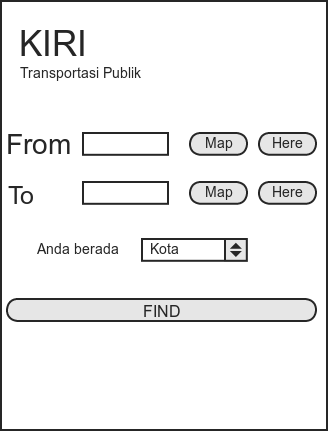
\includegraphics[scale=0.6]{Gambar/perancangan_antarmuka/Home}
	\caption{Antarmuka \textit{MainPage}}
	\label{fig:Antarmuka MainPage}
\end{figure}

\hspace{0.5cm} Antarmuka Kelas Map pada gambar ~\ref{fig:Antarmuka MainPage} merupakan tampilan awal saat aplikasi dijalankan. Antarmuka Kelas Map memiliki dua buah masukan, lima buah tombol, dan satu menu daftar. Berikut adalah detailnya.

Dua buah masukan yaitu.
\begin{itemize}
	\item Masukan lokasi asal\\
	Merupakan masukan lokasi asal mula pengguna ingin melakukan perjalanan.
	\item Masukan lokasi tujuan\\
	Merupakan masukan lokasi tujuan berhentinya perjalanan.
\end{itemize}

Lima buah tombol yaitu. 
\begin{itemize}
	\item Tombol map untuk lokasi asal\\
	Jika tombol ditekan maka akan berpindah ke kelas map untuk memilih lokasi asal di peta. Jika di kelas Map pengguna memilih lokasi maka pada masukan lokasi asal terdapat tulisan "Maps".
	\item Tombol here untuk lokasi asal\\
	Jika tombol ditekan maka lokasi asal adalah lokasi perangkat saat tombol ditekan dan masukan lokasi asal menjadi "here".
	\item Tombol map untuk lokasi tujuan\\
	Jika tombol ditekan maka akan berpindah ke kelas map untuk memilih lokasi tujuan di peta. Jika di kelas Map pengguna memilih lokasi maka pada masukan lokasi tujuan terdapat tulisan "Maps".
	\item Tombol here untuk lokasi tujuan\\
	Jika tombol ditekan maka lokasi tujuan adalah lokasi perangkat saat tombol ditekan dan masukan lokasi tujuan menjadi "here".
	\item Tombol find\\
	Jika tombol ditekan maka akan menampilkan daftar tempat asal dan tempat tujuan lalu mengarahkan ke Kelas Route.
\end{itemize}

Satu buah daftar yaitu.
\begin{itemize}
	\item Daftar kota yang tersedia\\
	Merupkan daftar kota yang tersedia (kota yang rute angkutan umumnya dapat ditemukan dengan aplikasi ini). Disaat aplikasi dijalankan maka daftar akan menunjuk ke kota terdekat tempat perangkat berada.
\end{itemize}

%Antarmuka list Tempat
\begin{figure}[h]
	\centering
		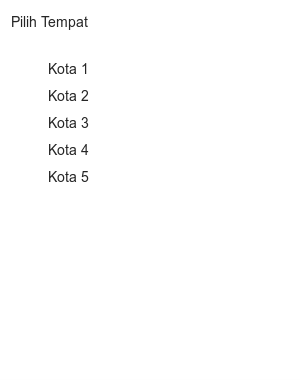
\includegraphics[scale=0.6]{Gambar/perancangan_antarmuka/ListTempat}
	\caption{Antarmuka Daftar Tempat}
	\label{fig:Antarmuka Daftar Tempat}
\end{figure}

\hspace{0.5cm} Antarmuka Daftar Tempat pada gambar ~\ref{fig:Antarmuka Daftar Tempat} merupakan daftar yang akan dimunculkan jika pengguna memasukan kata kunci pada pencarian tempat asal dan tempat tujuan. Daftar akan muncul jika didapat kembalian hasil pencarian lebih dari satu.

%Kelas Map
\subsection{Antarmuka Kelas \textit{Map}}
\label{lab:Antarmuka Kelas Map}

% Antarmuka Map
\begin{figure}[h]
	\centering
		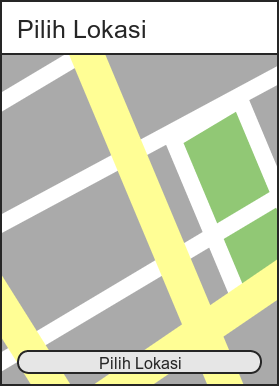
\includegraphics[scale=0.6]{Gambar/perancangan_antarmuka/Map}
	\caption{Antarmuka \textit{Map}}
	\label{fig:Antarmuka Map}
\end{figure}

\hspace{0.5cm} Antarmuka Kelas Map pada gambar ~\ref{fig:Antarmuka Map} merupakan antarmuka untuk menunjuk lokasi pada peta. Terdapat satu buah tombol yang akan dimunculkan jika pengguna sudah memilih lokasi. Jika tombol ditekan maka kordinat lokasi akan di simpan dan dikirim pada kelas MainPage dan halaman akan diarahkan ke kelas MainPage.

%Kelas Route
\subsection{Antarmuka Kelas \textit{Route}}
\label{lab:Antarmuka Kelas Route}

% Antarmuka route
\begin{figure}[h]
	\centering
		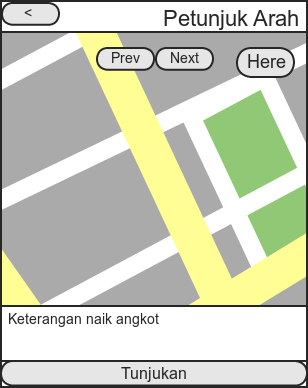
\includegraphics[scale=0.6]{Gambar/perancangan_antarmuka/Route}
	\caption{Antarmuka \textit{Route}}
	\label{fig:Antarmuka Route}
\end{figure}

\hspace{0.5cm} Antarmuka Kelas Route pada gambar ~\ref{fig:Antarmuka Route} merupakan antarmuka untuk melihat rute dari lokasi asal ke lokasi tujuan dalam bentuk daftar maupun peta. Terdapat empat buah tombol pada antarmuka Kelas Route. Berikut tombol yang terdapat pada Kelas Route. 
\begin{itemize}
	\item Tombol prev\\
	Jika tombol ditekan maka akan menunjuk titik sebelumnya pada rute peta.
	\item Tombol next\\
	Jika tombol ditekan maka akan menunjuk titik setelahnya pada rute peta.
	\item Tombol here\\
	Jika tombol ditekan maka akan menunjuk lokasi perangkat berada pada peta.
	\item Tombol Show List\\
	Jika tombol ditekan maka akan menunjuk atau menyembunyikan daftar rute.
\end{itemize}

% Antarmuka list route
\begin{figure}[h]
	\centering
		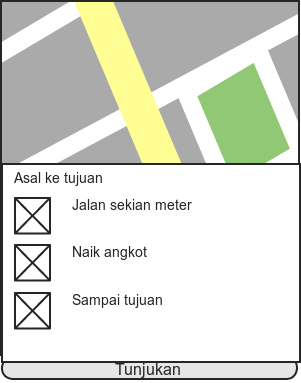
\includegraphics[scale=0.6]{Gambar/perancangan_antarmuka/ListRoute}
	\caption{Antarmuka Rute dalam bentuk Daftar}
	\label{fig:Antarmuka listRoute}
\end{figure}

\hspace{0.5cm} Antarmuka rute dalam bentuk daftar pada gambar ~\ref{fig:Antarmuka listRoute} merupakan antarmuka untuk melihat rute secara lebih jelas dengan keterangan tahap demi tahap disertai jarak dan waktu perjalanan. Antarmuka daftar dapat dilihat atau disembunyikan sesuai keinginan pengguna namun saat kelas Rute dibuka antarmuka daftar rute akan disembunyikan.